\documentclass[fr]{jdoc}

\usepackage[charter]{mathdesign}
\usepackage[colorlinks=true,urlcolor=blue]{hyperref} % hypertext links in color
\usepackage{xifthen}
\usepackage{tikz}
\usepackage{booktabs}
\usepackage{rotating}
\usepackage{multirow}
\usepackage{amsmath}
\usepackage{varwidth}
\usepackage{overpic}
\usepackage{lipsum}
\usepackage{xfrac}
\usepackage{pgfplots}
\usepackage{url}
\usepackage{subfigure}

\pgfplotsset{compat=1.8}
\usetikzlibrary{positioning, topaths, shapes, arrows, patterns}

\newcommand\newcite[2][]{\ifthenelse{\equal{#1}{}}{\citet{#2}}{\citet[#1]{#2}}}
\newcommand\TODO[1]{\textcolor{red}{[TODO #1]}}

\ed{PRES LUNAM\\École Doctorale STIM\\Sciences et Technologies de\\l'Information et Mathématiques}
\spec{Informatique}
\labo{LINA}
\equipe{TALN}

\title{Extraction automatique de termes-clés à partir de sujets}
\author{Adrien Bougouin}
\email{adrien.bougouin@univ-nantes.fr}

\begin{document}
  \makehead % builds header (ed, specialty, labo, title, author, ...).

  \begin{abstract}
    Les termes-clés sont les mots ou les expressions polylexicales, c'est-à-dire
    les séquences de mots grammaticalement correctes, qui représentent le
    contenu principal d'un document. Ils sont utiles pour diverses applications
    telles que l'indexation automatique de documents, mais ne sont pas toujours
    disponibles les documents. Dans cet article nous présentons TopicRank, une
    méthode à base de graphe pour l'extraction automatique de termes-clés. Cette
    méthode groupe les termes-clés candidats d'un document en sujets,
    représente le document par un graphe de sujets, ordonne les sujets selon
    leur importance au sein du graphe et extrait pour chacun des meilleurs
    sujets le terme-clé candidat qui le représente le mieux. L'expérience
    réalisée avec TopicRank montrent une amélioration significative vis-à-vis
    des méthodes à base de graphe existentes.
  \end{abstract}

  \begin{keywords}
    Extraction de termes-clés, méthode non-supervisée, méthode à base de graphe,
    groupement en sujets, ordonnancement de sujets.
  \end{keywords}

  \begin{collaborations}
    Projet ANR TermITH (ANR-12-CORD-0029).
  \end{collaborations}

  \section{Introduction}
\label{sec:introduction}
  % * définition de terme-clé, applications et enjeux
  Un terme-clé est un mot ou une expression polylexicale qui représente un
  concept important d'un document auquel il est associé. En pratique, plusieurs
  termes-clés représentant des concepts différents sont associés à un même
  document. Ils forment alors un ensemble de termes-clés à partir duquel il est
  possible de déduire le contenu principal du document. Du fait de leur capacité
  à synthétiser le contenu d'un document, les termes-clés sont utilisés dans
  diverses applications en Recherche d'Information (RI)~: résumé
  automatique~\cite{avanzo2005keyphrase}, classification de
  documents~\cite{han2007webdocumentclustering}, indexation
  automatique~\cite{medelyan2008smalltrainingset}, etc. Avec l'essor du
  numérique, de plus en plus de documents (articles scientifiques, articles
  journalistiques, etc.) sont accessibles depuis des médiums d'informations tels
  que Internet. Afin de permettre à un utilisateur de rapidement trouver des
  documents, ainsi que d'avoir un bref aperçu de leur contenu, les tâches
  sus-mentionnées sont nécessaires.
  Cependant, la majorité des documents ne sont pas associés avec des termes-clés
  et, compte tenu du nombre important de documents numériques, l'ajout manuel de
  ces derniers n'est pas envisageable. Pour pallier ce problème, de plus en plus
  de chercheurs s'intéressent à l'extraction automatique de termes-clés et
  certaines campagnes d'évaluations, telles que DEFT~\cite{paroubek2012deft} et
  SemEval~\cite{kim2010semeval}, proposent des tâches d'extraction automatique
  de termes-clés.

  % * qu'est-ce que l'extraction automatique de termes-clés
  % * deux écoles : indexation libre et indexation contrôlée (assignation de
  %                 termes-clés)
  %   -> nous sommes de la première école
  % * deux catégories de méthodes : supervisées et non-supervisées
  %    -> en supervisé ils utilisent la structure des documents
  %    -> très peu de travaux en non-supervisé (filtrage des candidats)
  L'extraction automatique de termes-clés, ou indexation libre, est la tâche qui
  consiste à extraire les unités textuelles les plus importantes d'un document,
  en opposition à la tâche d'assignation automatique de termes-clés, ou
  indexation contrôlée, qui consiste à assigner des termes-clés à partir d'une
  terminologie donnée~\cite{paroubek2012deft}. Parmi les méthodes d'extraction
  automatique de termes-clés existantes, nous distinguons deux catégories~: les
  méthodes supervisées et les méthodes non-supervisées. Dans le cas supervisé,
  la tâche d'extraction de termes-clés est considérée comme une tâche de
  classification binaire~\cite{witten1999kea}, où il s'agit d'attribuer la
  classe \og{}\textit{terme-clé}\fg{} ou \og{}\textit{non terme-clé}\fg{} aux
  termes-clés candidats extraits du document. Une collection de documents
  annotés en termes-clés est alors nécessaire pour l'apprentissage d'un modèle
  de classification reposant sur divers traits, allant de la simple fréquence
  aux informations structurelles du document (titre, résumé, introduction,
  conclusion, etc.). Dans le cas non-supervisé, les méthodes attribuent un
  score d'importance à chaque candidat en fonction de divers indicateurs tels
  que la fréquence et la position de la première occurrence dans le document.
  Bien que les méthodes supervisées soient en général plus performantes, la
  faible quantité de documents annotés en termes-clés disponibles, ainsi que la
  forte dépendance des modèles de classification au type des documents à partir
  desquels ils sont appris, poussent les chercheurs à s'intéresser de plus en
  plus aux méthodes non-supervisées.

  % * ici, on cherche à identifier l'échelle de difficulté d'indexation des
  %   documents en Sciences Humaines et Sociales (SHS)
  % * on dispose de 4 collections de notices de 4 disciplines différentes de
  %   SHS + 1 collection de notices de chimie (science dure)
  Dans cette article, nous nous intéressons à l'extraction non-supervisée de
  termes-clés dans les articles scientifiques, et plus particulièrement à la
  performance des méthodes d'extraction de termes-clés dans des domaines de
  spécialité. Au moyen de cinq corpus disciplinaires, notre objectif est
  d'observer et d'analyser l'échelle de difficulté pour l'extraction
  automatique de termes-clés dans des articles scientifiques appartenant à cinq
  disciplines différentes~: Archéologie, Sciences de l'Information,
  Linguistique, Psychologie et Chimie.
  \TODO{Dire pourquoi nous nous intéressons aux méthodes non-supervisées}
  \TODO{Dire pourquoi nous nous intéressons aux articles scientifiques}

  % * annonce du plan
  L'article est structuré comme suit. Un bref état de l'art est donné dans la
  section~\ref{sec:etat_de_l_art}, les données utilisées sont présentées dans la
  section~\ref{sec:presentation_des_donnees} et les expériences menées, ainsi
  que les résultats obtenus, sont décrits dans la section~\ref{sec:experiences}.
  Enfin, une analyse des résultats est donnée dans la
  section~\ref{sec:discussion}, puis une conclusion générale et des perspectives
  de travaux futurs sont présentés en
  section~\ref{sec:conclusion_et_perspectives}.


  \section{Extraction de termes-clés avec TopicRank}
\label{sec:extraction_de_termes_cles_avec_topicrank}
  \begin{itemize}
    \item{principe général}
    \item{identification des sujets}
    \item{ordonancement des sujets}
    \begin{itemize}
      \item{construction du graphe de sujets}
      \item{ordonnancement dans le graphe de sujets}
    \end{itemize}
    \item{selection des termes-clés}
  \end{itemize}


  \section{Experimental Settings}
\label{sec:experimental_settings}
  \subsection{Dataset}
  \label{subsec:dataset}
    In this work, we use the SemEval corpus. Built for the task 5 of
    SemEval-2010~\cite{kim2010semeval}, Sem\-Eval contains 244 English
    scientific papers collected from the ACM Digital Libraries. We use
    Sem\-Eval's training set (144 documents) and test set (100 documents) with
    their sets of combined author- and reader-assigned keyphrases.

  \subsection{Baselines}
  \label{subsec:baselines}
    In order to show that our method benefits from all aspects of its
    configuration, we design a set of baselines that slightly diverge from our
    method (deried baselines). First, To\-picRank plus the SVM classifier
    trained on either topically independent and dependent features
    (TopicRank+SVM), while the SVM classifier is trained on all features for our
    method (TopicRank+SVM$_{all}$). Second the SVM classifier, trained on either
    topically independent, dependent or all features, is applied to the unranked
    clusters (Clustering+SVM). Finally, the SVM classifier, trained on topically
    independent features, is applied candidate keyphrases (SVM).

    For comparison purpose, we also report results of a Naive Bayes classifier
    trained with the first position and the TF-IDF
    features~\cite[KEA]{witten1999kea}, TF-IDF and TopicRank.

  \subsection{Preprocessing}
  \label{subsec:preprocessing}
%    For each document, we apply the following preprocessing steps: sentence
%    segmentation, word tokenization and Part-of-Speech tagging. For sentence
%    segmentation, we use the PunktSentenceTokenizer provided by the Python
%    Natural Language ToolKit~\cite[NLTK]{bird2009nltk}. For word tokenization,
%    we use the NLTK TreebankWordTokenizer for English and the Bonsai word
%    tokenizer\footnote{The Bonsai word tokenizer is a tool provided with the
%    Bonsai PCFG-LA parser:
%    \url{http://alpage.inria.fr/statgram/frdep/fr_stat_dep_parsing.html}.} for
%    French. As for Part-of-Speech tagging, we use the Stanford POS
%    tagger~\cite{toutanova2003stanfordpostagger} for English and
%    MElt~\cite{denis2009melt} for French.
    %%%%%%%%%%%%%%%%%%%%%%%%%%%%%%%%%%%%%%%%%%%%%%%%%%%%%%%%%%%%%%%%%%%%%%%%%%%%
    For our method, as well as all baselines, we use Topic\-Rank's outputs.
    Therefore, our results can directly be compared to results
    in~\cite{bougouin2013topicrank}.

  \subsection{Evaluation Measures}
  \label{subsec:evaluation_measures}
    We evaluate the performances of our method and the baselines in terms of
    precision (P), recall (R) and f-score (f1-measure, F) when at most 10
    keyphrases are extracted. In order to reduce mismatches due to flexions such
    as plural, we also stem candidate and reference keyphrases during the
    evaluation.

\section{Results}
\label{sec:results}
  Figure~\ref{fig:baseline_comparison} presents the performance of our method,
  compared to six baselines derived from it. On the first hand, we observe that
  using clusters and their importance score benefits to the keyphrase
  extraction. Most importantly, adding topically dependent features to the
  common features improves the performance. However, the performance achieved
  with the Clustering+SVM method shows that topically dependent features
  performs poorly when Topic\-Rank's importance score is not used. Additionally,
  the SVM performance tends to show that using clusters without taking their
  importance into account is not relevant. Results support our statement that
  keyphrases should be extracted from important topics.
  \begin{figure}[h]
    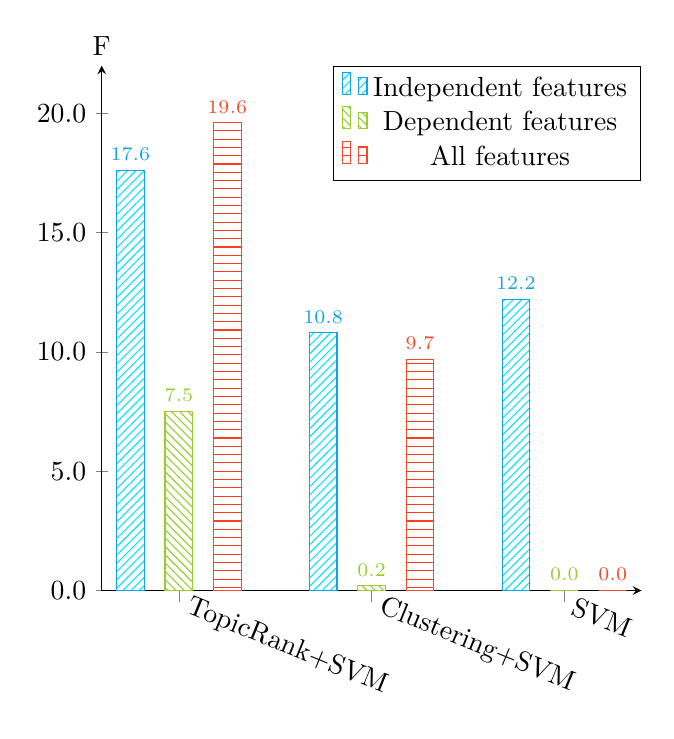
\begin{tikzpicture}%[scale=.75]
      \pgfkeys{/pgf/number format/.cd, fixed, fixed zerofill, precision=1}
      \begin{axis}[axis lines=left,
                   symbolic x coords={TopicRank+SVM, Clustering+SVM, SVM},
                   xtick=data,
                   enlarge x limits=0.2,
                   %x=.25\linewidth,
                   xticklabel style={anchor=west, rotate=-22.25},
                   nodes near coords,
                   nodes near coords align={vertical},
                   every node near coord/.append style={font=\scriptsize},
                   ytick={0.0, 5.0, 10.0, 15.0, 20.0, 25.0},
                   y=0.025\linewidth,
                   ymin=0.0,
                   ymax=22.0,
                   ybar=7.5pt,
                   ylabel=F,
                   ylabel style={at={(ticklabel* cs:1)},
                                 anchor=south,
                                 rotate=270},
                   legend style={at={(1.0, 1.0)},
                                 anchor=north east}]
        \addplot[Cerulean,
                 pattern=north east lines,
                 pattern color=Cerulean] coordinates{
          (SVM, 12.2)
          (Clustering+SVM, 10.8)
          (TopicRank+SVM, 17.6)
        };
        \addplot[YellowGreen,
                 pattern=north west lines,
                 pattern color=YellowGreen] coordinates{
          (SVM, 0.0)
          (Clustering+SVM, 0.2)
          (TopicRank+SVM, 7.5)
        };
        \addplot[RedOrange,
                 pattern=horizontal lines,
                 pattern color=RedOrange] coordinates{
          (SVM, 0.0)
          (Clustering+SVM, 9.7)
          (TopicRank+SVM, 19.6)
        };
        \legend{Independent features, Dependent features, All features}
      \end{axis}
    \end{tikzpicture}
    \caption{Performance of TopicRank+SVM$_{all}$ compared to derived baselines
             \label{fig:baseline_comparison}}
  \end{figure}

  Also, Table~\ref{tab:state_of_the_art_comparison} presents a comparison of
  TopicRank+SVM$_{all}$ with TopicRank, TopicRank's best possible performance
  (TopicRank$_{max}$) and common baselines of previous work. Results show that
  our method significantly improves TopicRank and significantly outperform
  TF-IDF and KEA, a robust supervised methods. However, the performance of
  TopicRank+SVM$_{all}$ is still very low compared to the best possible
  performance that could be achieved with TopicRank. The naivety of the
  clustering method TopicRank applies may introduce noise that dampens the
  performance. Future improvement should focus on a more efficient clustering of
  the candidates belonging to the same topic.
  \begin{table}[h]
    \centering
    \begin{tabular}{|r|rrr|}
      \hline
      Method & \multicolumn{1}{c}{P} & \multicolumn{1}{c}{R} & \multicolumn{1}{c|}{F}\\
      \hline
      KEA                   & 18.8\textcolor{white}{$^\dagger$} & 13.3\textcolor{white}{$^\dagger$} & 15.4\textcolor{white}{$^\dagger$}\\
      TF-IDF                & 13.2\textcolor{white}{$^\dagger$} & 8.9\textcolor{white}{$^\dagger$} & 10.5\textcolor{white}{$^\dagger$}\\
      TopicRank             & 14.9\textcolor{white}{$^\dagger$} & 10.3\textcolor{white}{$^\dagger$} & 12.1\textcolor{white}{$^\dagger$}\\
      TopicRank+SVM$_{all}$ & 24.2$^\dagger$ & 16.7$^\dagger$ & 19.6$^\dagger$\\
      \hline
      TopicRank$_{max}$     & 37.6\textcolor{white}{$^\dagger$} & 25.8\textcolor{white}{$^\dagger$} & 30.3\textcolor{white}{$^\dagger$}\\
      \hline
    \end{tabular}
    \caption{Performance of TopicRank+SVM$_{all}$ compared to previous work.
      $\dagger$ indicates improvement over KEA, TF-IDF and TopicRank at 0.001
      level using Student's t-test.
             \label{tab:state_of_the_art_comparison}}
  \end{table}

%\section{Error Analysis}
%\label{sec:error_analysis}


  \section{Conclusion et perspectives}
\label{sec:conclusion_et_perspectives}
  Dans cet article, nous nous intéressons à la tâche d'extraction automatique de
  termes-clés dans les documents scientifiques et émettons l'hypothèse que sa
  difficulté est variable selon la discipline des documents traités. Pour
  vérifier cette hypothèse, nous disposons de notices bibliographiques réparties
  dans cinq disciplines (archéologie, linguistique, sciences de l'information,
  psychologie et chimie) auxquelles nous appliquons six systèmes d'extractions
  automatique de termes-clés différents. En comparant les termes-clés extraits
  par chaque système avec les termes-clés de référence assignés aux notices dans
  des conditions réels d'indexation, notre hypothèse se vérifie et nous
  observons l'échelle suivante (de la discipline la plus facile à la plus
  difficile)~:
  \begin{enumerate*}
    \item{Archéologie~;}
    \item{Linguistique~;}
    \item{Sciences de l'information~;}
    \item{Psychologie~;}
    \item{Chimie.}
  \end{enumerate*}

  À l'issue de nos expériences et de nos observations du contenu des notices,
  nous constatons deux facteurs ayant un impact sur la difficulté de la tâche
  d'extraction automatique de termes-clés. Tout d'abord, nous observons que
  l'organisation du résumé peut aider l'extraction de termes-clés. Un résumé
  riche en explications et en mises en relations des différents concepts est
  moins difficile à traiter qu'un résumé énumératif pauvre en explications.
  Ensuite, le vocabulaire utilisé dans une discipline peut influer sur la
  difficulté à extraire les termes-clés des documents de cette discipline. Si le
  vocabulaire spécifique contient des composés syntagmatiques dont certains
  éléments sont courants dans la discipline, alors il peut être plus difficile
  d'extraire les termes-clés des documents de cette discipline.

  Des deux facteurs identifiés émergent plusieurs perspectives de travaux
  futurs. Il peut être intéressant d'analyser le discours des documents afin de
  mesurer, en amont, le degré de difficulté de l'extraction de termes-clés. Avec
  une telle connaissance, nous pourrions proposer une méthode capable de
  s'adapter au degré de difficulté en ajustant automatiquement son paramètrage.
  Cependant, l'analyse que nous proposons dans cet article se fonde uniquement
  sur le contenu de notices appartenant à cinq disciplines. Il serait pertinent
  d'étendre cette analyse au contenu intégral des documents scientifiques, ainsi
  que d'élargir le panel de disciplines utilisées dans ce travail, afin
  d'établir des catégories de discplines plus ou moins difficiles à traiter
  (p.~ex. la chimie fait partie des disciplines expérimentales, qui sont
  difficiles à traiter). Nous oberservons aussi que le vocabulaire utilisé dans
  une discipline, en particulier celui utilisé pour les termes-clés, peut rendre
  la tâche d'extraction automatique de termes-clés plus difficile. Il est donc
  important de bénéficier de resources telles que des thésaurus pour permettre à
  une méthode d'extraction de termes-clés de s'adapter au domaine. Pour
  TopicRank, par exemple, avoir connaissance de la terminologie utilisée dans
  une discipline peut améliorer le choix du terme-clé le plus représentatif d'un
  sujet. Enfin, il serait intéressant de penser la tâche d'extraction de
  termes-clés comme une tâche d'extraction d'information pour le remplissage
  d'un formulaire. En archéologie, par exemple, il pourrait s'agir d'extraire
  les informations géographiques (pays, régions, etc.), chronologiques (période,
  culture, etc.), ou encore environnementales (animaux, végétaux, etc.).



  \bibliography{../../biblio}
\end{document}

